\documentclass[11pt]{article}

\usepackage[letterpaper,margin=1in]{geometry}

% ToC
\usepackage{blindtext} 
\usepackage[linktocpage]{hyperref}
\usepackage{bookmark}
\usepackage[compact]{titlesec}

% bib
%\usepackage[round]{natbib}
\usepackage[square,sort,numbers]{natbib}

% Math Imports
\usepackage{amsmath, amssymb, bm, fancyhdr, sectsty, dsfont, mathtools}

% Tikz
\usepackage{tikz}
\usetikzlibrary{bayesnet}
\usetikzlibrary{arrows}

\usepackage{wrapfig}
\usepackage{comment}
\usepackage{subcaption}

% Symbols
\newcommand\ind{\protect\mathpalette{\protect\independenT}{\perp}}
\def\independenT#1#2{\mathrel{\rlap{$#1#2$}\mkern2mu{#1#2}}}
\newcommand\norm[1]{\left\lVert#1\right\rVert}
\newcommand\set[1]{\left\{#1\right\}}

\newcommand\RNN{\mathrm{RNN}}
\newcommand\MLP{\mathrm{MLP}}
\newcommand\enc{\mathrm{enc}}
\newcommand\softmax{\mathrm{softmax}}

% Distributions
\newcommand{\Cat}{\mathrm{Cat}}
\newcommand\Expo{\mathrm{Expo}}
\newcommand\Bern{\mathrm{Bern}}
\newcommand\Pois{\mathrm{Pois}}
\newcommand\Bin{\mathrm{Bin}}
\newcommand\Unif{\mathrm{Unif}}
\newcommand\Betad{\mathrm{Beta}}
\newcommand\Gammad{\mathrm{Gamma}}
\newcommand\Geom{\mathrm{Geom}}
\newcommand\Logd{\mathrm{Logistic}}

\newcommand\E[1]{\mathbb{E}\left[#1\right]}
\newcommand\Es[2]{\mathbb{E}_{#1}\left[#2\right]}
\newcommand{\Var}{\mathrm{Var}}
\newcommand{\Cov}{\mathrm{Cov}}
\newcommand{\Cor}{\mathrm{Cor}}

% Bold stuff
\newcommand{\ba}{\mathbf{a}}
\newcommand{\bb}{\mathbf{b}}
\newcommand{\bc}{\mathbf{c}}
\newcommand{\bd}{\mathbf{d}}
\newcommand{\be}{\mathbf{e}}
\newcommand{\bg}{\mathbf{g}}
\newcommand{\bh}{\mathbf{h}}
\newcommand{\br}{\mathbf{r}}
\newcommand{\bs}{\mathbf{s}}
\newcommand{\bw}{\mathbf{w}}
\newcommand{\bx}{\mathbf{x}}
\newcommand{\by}{\mathbf{y}}
\newcommand{\bz}{\mathbf{z}}

% mathcal stuff
\newcommand{\mcD}{\mathcal{D}}

% math blackboard bold stuff
\newcommand{\R}{\mathbb{R}}
\newcommand{\C}{\mathbb{C}}
\newcommand{\Z}{\mathbb{Z}}
\newcommand{\N}{\mathbb{N}}
\newcommand{\Q}{\mathbb{Q}}


\DeclareMathOperator*{\argmin}{argmin}
\DeclareMathOperator*{\argmax}{argmax}

\titlespacing{\paragraph}{0pt}{*0}{*0}
%\setlength{\parskip}{-5mm plus1mm minus1mm}

\usepackage{fancyhdr}
\pagestyle{fancy}


\begin{document}
\lhead{Justin Chiu}
\chead{2018 NSF GRFP}
\rhead{Research Proposal}

\begin{center}
\textbf{Latent Variable Models for Data to Text}
\end{center}

\paragraph{Keywords}
latent variable models, conditional text generation, data to text

\paragraph{Background}
Natural language processing (NLP) can largely be decomposed into two separate but
tightly related tasks: natural language understanding and natural language generation (NLG).
In this proposal we focus primarily on generation, and in particular
the generation of text that describes some data.
We refer to this specific task as Data-to-Text (D2T).
The assumption that the text describes data is central to the task as it allows for practitioners to 
define heuristics for evaluatating a summary's fidelity to the underlying data.

%\paragraph{Why is D2T important?}
% Easily evaluable, good benchmark
% Limited external knowledge
% Largely concerned with reporting the information in the table
The D2T task's importance is two-fold.
First, D2T serves as a useful benchmark for conditional generation.
D2T exists as a compromise between short-form generative tasks such as sentence-level translation
and unstructured long-form tasks such as generating Wikipedia articles from internet resources.
This is because D2T is a long-form generation task but uses structured data as input instead of free-form text.
Secondly, the existence of structured data represents a simplifying assumption which makes D2T easier than other
long-form tasks but also, more importantly, amenable to automatic evaluation.
Given a list of records and the assumption that in a data-text pair the text's purpose is to describe the data,
it is straightforward to obtain approximate alignments between the text and records for evaluation.
However, the alignments can also be used for much more than evaluation; they can be used for obtaining weak supervision
\citep{puduppully2018contentselection}. %in a latent variable model.
This insight motivates our proposal and will be elaborated on shortly.

Early work on D2T focused on the use of templates and grammars framed as latent variable models, 
which generally resulted in generations with little stylistic variation.
% Do I need to qualify this claim and say why?
After neural language models demonstrated state of the art performance,
they were then transferred to the conditional language modeling setting,
i.e. D2T and more broadly NLG,
where they supplanted template-based methods almost completely.
However, by relying largely on the language modeling capabilities of neural networks,
practitioners have eschewed modularity of the model for ease of inference.
% Do I need to qualify this as well?
\citep{angeli2010d2t}, \citep{liang2009semalign}, \citep{sauper2009wiki}

\paragraph{Research Question}
%We can train end-to-end modular systems, so how much modularity and supervision can we provide and does it help the model?
As research on D2T has embraced neural systems and end-to-end training resulting in very unstructured models,
what is the benefit of imbuing more structure in the form of a latent variable model?

% Proposal? Add more structure / modularity, principled inference...?
% Thesis: structure will help with controllability and LVM formulation with generalization as it presents a different inductive bias?
\paragraph{Research}

\paragraph{Data}
% Example of D2T, should i present this early or later
The dataset we consider primarily is the Rotowire dataset \citep{wiseman2017d2t},
where a summary of a basketball game is modelled conditioned on the box score associated with that game.
This is the most recent D2T dataset that has been developed.
The box score consists of a list of records associating an entity with a value.
Each record has a type which denotes the relationship between the entity and value contained in the record.
An example record could look like: (type = POINTS, entity = Jeremy Lin, value = 19).

\paragraph{What are the desiderata of a text generation system?}
\begin{enumerate}
\item Readability: Fluency, grammaticality, interestingness?
\item Controllability, ability to impose constraints
\item Fidelity to conditioning
\item What does interpretability mean here?
\item Informational adequacy: Can we learn what records are salient?
\end{enumerate}

A vein in the recent work on integrating neural network systems and latent variable models
has aimed to separate content from style.
Separate style and content, where content will come from for controllable generation.
Can we also model intention in a similar way?
Hierarchical planning, multiple levels
cite fair thing with dialogue planning? 

\paragraph{Related Work}
In the task of generating basketball summaries from game statistics,
\citet{puduppully2018contentselection} learn a model of content progression
by learning how to order records from the table of statistics.
\citep{puduppully2018contentselection,wiseman2018template}
Separate content from style
\paragraph{Approach and Methods}

\begin{wrapfigure}{r}{0.5\textwidth}
\centering
\begin{subfigure}[]{0.5\textwidth}
\centering
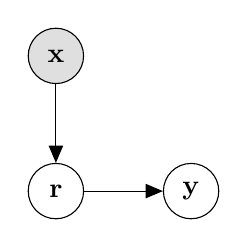
\begin{tikzpicture}
\node(x)[obs]{$\bx$};
\node(r)[latent, below =of x]{$\br$};
\node(y)[latent, right =of r]{$\by$};
\edge {x} {r};
\edge {r} {y};
\end{tikzpicture}
\caption{}
\end{subfigure}

\begin{comment}
\hspace{0.03\textwidth}
\begin{subfigure}[]{0.3\textwidth}
\centering
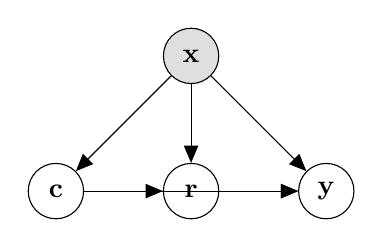
\begin{tikzpicture}
\node(x)[obs]{$\bx$};
\node(r)[latent, below =of x]{$\br$};
\node(c)[latent, left =of r]{$\bc$};
\node(y)[latent, right =of r]{$\by$};

\edge {x} {c};
\edge {x} {r};
\edge {x} {y};
\edge {c} {r};
\edge [bend right=45] {c} {y};
\edge {r} {y};

\end{tikzpicture}
\caption{}
\end{subfigure}
\hspace{0.03\textwidth}
\end{comment}

\begin{comment}
% Noisy channel model
\begin{subfigure}[]{0.3\textwidth}
\centering
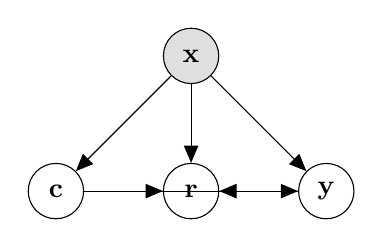
\begin{tikzpicture}
\node(x)[obs]{$\bx$};
\node(r)[latent, below =of x]{$\br$};
\node(c)[latent, left =of r]{$\bc$};
\node(y)[latent, right =of r]{$\by$};

\edge {x} {c};
\edge {x} {r};
\edge {x} {y};
\edge {c} {r};
\edge [bend right=45] {c} {y};
\edge {y} {r};
\end{tikzpicture}
\caption{}
\end{subfigure}
\end{comment}

\begin{subfigure}[]{0.3\textwidth}
\centering
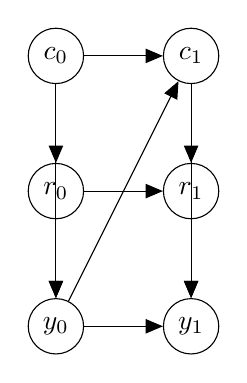
\begin{tikzpicture}
\node(c0)[latent]{$c_0$};
\node(r0)[latent, below =of c0]{$r_0$};
\node(y0)[latent, below =of r0]{$y_0$};
\node(c1)[latent, right =of c0]{$c_1$};
\node(r1)[latent, below =of c1]{$r_1$};
\node(y1)[latent, below =of r1]{$y_1$};

\edge {c0} {r0};
\edge [bend right=45] {c0} {y0};
\edge {r0} {y0};

\edge {c1} {r1};
\edge [bend left=45] {c1} {y1};
\edge {r1} {y1};

\edge {c0} {c1};
\edge {r0} {r1};
\edge {y0} {y1};

\edge {y0} {c1};

\end{tikzpicture}
\caption{}
\end{subfigure}
\label{fig:dgm}
\caption{Simplistic directed graphical models for the latent variable model.
The observed context is $\tilde\bx$, current attention $a_t$, previous attention $a_{t-1}$,
state $s_t$, and target word $y_t$.}
\end{wrapfigure}

\begin{figure}[ht]
\label{fig:dgm2}
\caption{The time-series graphical model.
As all nodes condition on $\bx$, we omit it from the diagram.}
\end{figure}

\paragraph{Intellectual Merit}
\paragraph{Broader Impact}


\bibliographystyle{plainnat}
\bibliography{w}


\end{document}

